\documentclass[UTF8]{ctexart}
\hfuzz=4pt

\usepackage{parskip}
    \setlength{\parindent}{0em}
    \setlength{\parskip}{1em}
\usepackage{geometry}
    \geometry{left=4cm,right=4cm,top=2cm,bottom=2cm}
\usepackage{amsmath, amssymb, amsthm, mathtools}
\usepackage{thmtools}
    \renewcommand\qedsymbol{$\blacksquare$}
    \declaretheorem[numberwithin=section,shaded={rulecolor=cyan,rulewidth=2pt,bgcolor=white}]{definition}
    \declaretheorem[numberwithin=section,shaded={rulecolor=orange,rulewidth=2pt, bgcolor=white}]{theorem} 
    \newtheoremstyle{mystyle}{1em plus .2 em minus .2em}{1em plus .2 em minus .2em}{}{}{\bfseries}{.}{.5em}{}
    \theoremstyle{mystyle}
    \newtheorem{axiom}{Axiom}[section]
    \newtheorem{lemma}{Lemma}[section]
    \newtheorem{proposition}{Proposition}[section]
    \newtheoremstyle{myremark}{1em plus .2 em minus .2em}{1em plus .2 em minus .2em}{}{}{\itshape}{.}{.5em}{}
    \theoremstyle{myremark}
    \newtheorem*{remark}{Remark}
    \theoremstyle{plain}
    \newtheorem{corollary}{Corollary}[section]
\usepackage{caption}
\usepackage{xcolor}
\usepackage{graphicx}
\usepackage{float}
\usepackage{setspace} 	 % 行间距 \begin{spacing}{arg}
\usepackage{esint}
\usepackage{hyperref}
    \hypersetup{colorlinks=true,linktoc=all,linkcolor=blue}

\newcommand{\ve}[1]{\boldsymbol{\mathbf{#1}}}
\newcommand{\unit}[1]{\boldsymbol{\mathbf{\hat{#1}}}}
\renewcommand{\r}{\mathrm}
\renewcommand{\cal}{\mathcal}
\newcommand{\scr}{\mathscr}

\newcommand{\E}{\mathrm e}
\renewcommand{\I}{\mathrm i}
\newcommand{\R}{\mathbb R}
\newcommand{\Z}{\mathbb Z}
\newcommand{\N}{\mathbb N}
\newcommand{\Q}{\mathbb Q}
\renewcommand{\C}{\mathbb C}
\DeclarePairedDelimiter\set{\{}{\}}
\def \DD #1.#2.#3 {\dfrac{d^{#1} #2}{d #3^{#1}}}
\def \PP #1.#2.#3 {\dfrac{\partial^{#1} #2}{\partial #3^{#1}}}
\def \dd #1.#2 {\dfrac{d #1}{d #2}}
\def \pp #1.#2 {\dfrac{\partial #1}{\partial #2}} 
\newcommand{\del}{\nabla}
\DeclareMathOperator{\dom}{dom}
\DeclareMathOperator{\range}{range}


\pagestyle{empty}

\begin{document}
\section{二元关系}
\subsection{关系的定义}
集合 $ A $ 到 $ B $ 的一个二元关系 $ R $ 是 $ A \times B $ 的子集, 可以看作是函数的推广.

\paragraph{例}
$ A = \set{a, b} $, $ B = \set{1, 2} $. 则 $ A \times B = \set{(a, 1), (a, 2), (b, 1), (b, 2)} $. 任取 $ A \times B $ 的一个子集, 就是 $ A $ 到 $ B $ 的一种关系: 如 $ R = \set{(a, 1), (b, 1)} $ 或 $ \set{(a, 1), (a, 2)} $.

和部分函数类似, $ A $ 到 $ B $ 的关系, 不代表 $ A $ 中每个元素都有 $ B $ 中对应关联的元素. 如果 $ A $ 中每个元素都能在 $ B $ 中找到元素和该元素存在关系, 则称这个关系为左完全的 (left-total) 或是连续的 (serial). 

\paragraph{例}
$ A = \set{a, b} $, $ B = \set{1, 2} $. 则关系 $ R_1 = \set{(a, 1), (b, 1)} $ 是左完全的, 因为 $ A $ 中所有元素, 都有 $ B $ 中对应存在关系的元素. 而关系 $ R_2 = \set{(a, 1), (a, 2)} $ 就不是左完全的, 因为在 $ B $ 中没有任何与 $ b \in A $ 存在关系的元素.

将函数中定义域的概念推广到关系中来, 定义 $ A $ 到 $ B $ 的关系 $ R $ 的定义域为 $ A $ 中存在关系的元素集
\[ 
    \dom R \coloneqq \set{a \in A \mid \exists b \in B, a R b }\,.
\]
所以一个关系 $ R \subseteq A \times B $ 为左完全的, 当且仅当 $ \dom R = A $.

$ f \colon A \to B $ 如果是一个部分函数, 那么我们可以把定义域限制到 $ A $ 中有定义的那部分上. 同理, 如果 $ A $ 到 $ B $ 的关系 $ R $ 不是左完全的, 那么我们可以限制 $ A $ 到它的子集 $ C $ 上, 得到新的关系, 记作 $ R|_C $ 或 $ R \restriction _C $. 所以如果我们限制一个不是左完全的关系 $ R $ 到其定义域上 $ R|_{\dom R} $, 则关系也就成为左完全的.

如上例中, $ A $ 到 $ B $ 的关系 $ R_2 = \set{(a, 1), (a, 2)} $ 不是左完全的, 但 $ \set{a} $ 到 $ B $ 的关系 $ R_2 |_{\set{a}} $ 是左完全的.

由于关系是函数的一种推广, 可以看作是允许一对多的``函数'', 大多数函数中的概念都可以引入到关系中来.

\subsection{关系的复合及性质}
\begin{definition}[\text{关系的复合}]
    设集合 $ A $ 到 $ B $ 的关系 $ R $, 以及 $ B $ 到 $ C $ 的关系 $ S $. 则 $ R $ 与 $ S $ 的复合 $ S \circ R $ 定义为:
    \[ S \circ R \coloneqq \set{(a, c) \mid \exists b \in B \text{ 使得 } (a, b) \in R \land (b, c) \in S} \,.\] 也可以采用记号 $ R;S $ 或 $ (R;S) $ 表示 $ R $ 与 $ S $ 复合.
\end{definition}

\begin{remark}
    用 $ \circ $ 表示复合也是借用函数复合的记号, 所以其顺序也遵循函数复合, 从右向左: 复合函数 $ g \circ f $ 表示先 $ f $ 后 $ g $. 复合关系 $ S \circ R $ 表示先 $ R $ 后 $ S $. 而使用分号 $ R;S $ 或 $ (R;S) $ 作为后来定义的记号, 则是从左向右, 以方便阅读. 两种方式 $ S \circ R $ 和 $ R;S $ 只是记号上的不同, 均代表相同含义: $ R $ 与 $ S $ 复合.
\end{remark}


\begin{proposition}[\text{复合的性质}] \ 
    \begin{itemize}
        \item (结合律) $ (R \circ S) \circ T = R \circ (S \circ T) $
        \item (恒等关系) $ R \circ I_A = R $,\quad $ I_A \circ R = R $
        \item (逆关系) $ R^{-1} \circ R = I_A|_R $,\quad $ R \circ R^{-1} = I_A|_{R^{-1}} $
        \item $ (R \circ S)^{-1} = S^{-1} \circ R^{-1} $
    \end{itemize}
\end{proposition}

特别要注意: $ R^{-1} \circ R $ 不一定等于 $ I_A $, 不要套用实数的幂法则 $ x^{-1} x = x^0 = 1 $. 


递归地定义 $ R^n $:
\[ R^n \coloneqq \begin{cases}
    I_A & n = 0 \\
    R^{n - 1} \circ R & n > 0
\end{cases} \,.\]

于是有:
\[ \begin{array}{c}
    R^0 = I_A \\
    R^1 = I_A \circ R = R \\
    R^2 = R^1 \circ R = R \circ R \\
    R^3 = R^2 \circ R = R \circ R \circ R
\end{array} \]

同时有下面关系:
\[ \begin{array}{c}
    \forall m,n \in \N, R^m \circ R^n = R^{m + n} \,, \\
    \forall m,n \in \N, \bigl( R^m \bigr)^n = R^{mn} \,.
\end{array} \]
务必牢记, 上面的幂的指数都是定义在自然数内的, 并没有拓广到整数集上.

\begin{proposition}
    对任意自然数 $ n $, $ \bigl( R^n \bigr)^{-1} = \bigl( R^{-1} \bigr)^n $. 
\end{proposition}

\begin{proof}
    通过归纳法, $ \bigl( R^{-1} \bigr)^1 = \bigl( R^1 \bigr)^{-1} $. 现归纳地假设 $ \bigl( R^{-1} \bigr)^n = \bigl( R^n \bigr)^{-1} $.
    \begin{align*}
        \bigl( R^{-1} \bigr)^{n + 1} &= \bigl( R^{-1} \bigr)^n \circ R^{-1} \\
        &= \bigl( R^n \bigr)^{-1} \circ R^{-1} \\
        &= \bigl( R \circ R^n \bigr)^{-1} \\
        &= \bigl( R^{n + 1} \bigr)^{-1} \,.
    \end{align*}
\end{proof}


\begin{theorem}[\text{传递性}]
    集合 $ A $ 上的关系 $ R $ 具有传递性, 当且仅当 $ R^n \subseteq R $ 对任意 $ n \in \Z^+ $ 均成立.
\end{theorem}

\begin{proof} \ \\
    正推: $ R^n \subseteq R $ 在 $ n = 1 $ 时成立, 此为基础情形. 现归纳地假设对于 $ n \geqslant 1 $, $ R^n \subseteq R $. 要证明 $ R^{n + 1} \subseteq R $. 对于 $ (a, b) \in R^{n + 1} $, 存在 $ c \in A $, $ (a, c) \in R^n $, $ (c, b) \in R $. 根据归纳假设, $ (a, c) $ 也一定在 $ R $ 中. 于是 $ (a, c) \in R $ 且 $ (c, b) \in R $, 由于传递性, $ (a, b) \in R $, 所以 $ R^{n + 1} \subseteq R $.
    
    反推: 设 $ R^n \subseteq R $ 对任意整数 $ n \geqslant 1 $ 成立. 若 $ (a, b) \in R $ 且 $ (b, c) \in R $, 则有 $ (a, c) \in R^2 $, 而 $ R^2 \subseteq R $, 所以 $ (a, c) \in R $. 这说明了传递性.
\end{proof}


\begin{proposition}
    设 $ R $ 为 $ A $ 上的关系:
    \begin{enumerate}
        \item $ R $ 是对称的 $ \iff $ $ R = R^{-1} $
        \item $ R $ 是反对称的 $ \iff $ $ R \cap R^{-1} \subseteq I_A $
        \item $ R $ 是自反的 $ \iff $ $ R^{-1} $ 自反
        \item $ R $ 是自反的 $ \iff $ $ \overline R $ 自反
    \end{enumerate}
\end{proposition}

\begin{proposition}
    $ R $ 是自反/对称关系, 则对任意正整数 $ n $, $ R^n $ 也是自反/对称的.
\end{proposition}

\begin{proposition}
    $ R $ 是自反和传递的关系, 则对任意正整数 $ n $, $ R^n = R $.
\end{proposition}

\begin{proof}
    一方面, $ R $ 是传递的, 根据传递性定理, $ R^n \subseteq R $ 对任意正整数 $ n $ 成立. 另一方面, $ R $ 是自反的, 可以通过归纳法证明 $ R \subseteq R^n $ 对任意 $ n $ 成立(注意应用自反的条件). 所以对任意 $ n \in \Z^+ $, $ R^n = R $.
\end{proof}

\subsection{关系的数量}
$ n $ 个元素任意选取的情况一共有 $ 2^n $ 个. 可以这样理解, 对于每个元素, 都有选或不选两种情况, 于是根据乘法公式, 选取的情况共有 $ n \cdot n \cdots n = 2^n $ 个. 此外, 这还可以从组合公式中看出: \[ \sum_{k = 0}^n \binom{n}{k} = \binom{n}{0} + \binom{n}{1} + \cdots + \binom{n}{n} = 2^n \,.\] 

\begin{proposition}
    $ n $ 元素集 $ A $ 上的自反关系有 $ 2^{n^2 - n} $ 个, 反自反关系也有 $ 2^{n^2 - n} $ 个.
\end{proposition}

\begin{proof}
    自反的条件为 $ \forall a \in A \bigl( (a, a) \in R \bigr) $. 所以关系矩阵的对角线必然全为 $ 1 $. 那么从剩下的 $ n^2 - n $ 个元素中选取任意元素置 $ 1 $, 得到的都为自反关系, 而这样的选取有 $ 2^{n^2 - n} $ 种. 反自反关系同理. 
\end{proof}

\begin{proposition}
    $ n $ 元素集上的对称关系有 $ 2^{(n^2 + n) / 2} $ 个.
\end{proposition}

\begin{proof}
    对称关系在关系矩阵中反应为关于对角线对称的元素相等. 故先选对角线任意一侧 (除开对角线上的元素), 这样的元素有 $ (n^2 - n) / 2 $ 个, 选取方法有 $ 2^{(n^2 - n) / 2} $ 种.

    再任意选取对角线上的元素, 因为对角线上的元素一定满足对称性. 故有 $ 2^n $ 种情况.

    两种选取情况相乘 $ 2^{(n^2 - n) / 2} \cdot 2^{n} $ 就得到结果.
\end{proof}

\begin{proposition}
    $ n $ 元素集上反对称关系有 $ 2^n 3^{(n^2-n)/2} $ 个. 非对称关系有 $ 3^{(n^2-n)/2} $ 个.
\end{proposition}

\begin{proof}
    对于选取出的 $ (a, b) \in R $ 和 $ (b, a) \in R $, 会导致 $ a = b $. 故选择对角线的情况有 $ 2^n $ 种.

    而如果选择出的 $ (a, b) $ 和 $ (b, a) $ 不同时满足关系 $ R $, 则有 $ 3 $ 种情况, 两者都不满足关系($ 1 $ 种)和两者中有一个满足关系($ 2 $ 种). 从对角线的任意一侧选择出元素, 有 $ (n^2 - n)/2 $ 个元素, 每个元素又有 $ 3 $ 种情况: 这个元素满足 $ R $ 但对称的元素不满足; 这个元素不满足但对称的元素满足; 这个元素和对称的元素都不满足. 所以一共有 $ 3^{(n^2 - n)/2} $ 种情况.

    第二次的选择数量就对应了非对称关系的数量 $ 3^{(n^2 - n)/2} $, 而反对称则是两次选择相乘: $ 2^n 3^{(n^2-n)/2} $.
\end{proof}


\begin{definition}[\text{贝尔数}]
    $ n $ 元集合上的划分情况有 $ B_n $ 种, 其中 $ B_n $ 为第 $ n $ 个贝尔数, 递归定义如下: \[ B_{n+1} = \sum_{k=0}^{n} \binom{n}{k} B_k \,.\] 前 $ 5 $ 个贝尔数如下: $ B_0 = B_1 = 1 $, $ B_2 = 2 $, $ B_3 = 5 $, $ B_4 = 15 $, $ B_5 = 52 $.
\end{definition}


\begin{proposition}
    $ n $ 元素集上的等价关系对应集合的一个划分, 故等价关系的数量为 $ B_n $.
\end{proposition}

\section{二元关系的表示}
使用矩阵描述二元关系, 当两个元素存在关系时, 矩阵对应元素为 $ 1 $, 否则为 $ 0 $.
\begin{definition}[\text{关系矩阵}]
    $ A = \set{x_i \mid 1 \leqslant i \leqslant n} $, $ B = \set{b_i \mid 1 \leqslant i \leqslant m} $. 设 $ R \subseteq A \times B $ 为 $ A $ 到 $ B $ 的关系. 定义该关系的关系矩阵 $ \ve M_R = (r_{ij})_{n \times m} $ 为
    \[ r_{ij} = \begin{cases}
        1  & (a_i, b_j) \in R \\
        0  & (a_i, b_j) \notin R
    \end{cases} \,.\]
\end{definition}

\paragraph{逆关系的关系矩阵}
根据定义, 下面的事实是显然的:
\[ 
    \ve M_{R^{-1}} = \ve M_R^\top \,.
\]

\paragraph{布尔积}
和关系矩阵相关的运算为布尔积 $ \odot $, 该运算作用与两个布尔矩阵上, 返回一个布尔矩阵. 对于 $ \ve A_{n \times m} $ 和 $ \ve B_{m \times p} $, 其布尔积的第 $ i $ 行 $ j $ 列如下:
\begin{align*}
    (\ve A \odot \ve B)_{ij} &= \bigvee_{\gamma = 0}^{m} \ve A_{i \gamma} \land \ve B_{\gamma j} \\
    &= (\ve A_{i1} \land \ve B_{1j}) \lor (\ve A_{i2} \land \ve B_{2j}) \lor \cdots \lor (\ve A_{im} \land \ve B_{mj}) \,.
\end{align*}

实际就是将一般矩阵乘法中, 数与数的乘法换成逻辑运算中对应的与运算, 同时将加法换成对应的或运算. 下面是一般的矩阵乘法.
\begin{align*}
    (\ve A \ve B)_{ij} &= \sum_{\gamma = 0}^{m} \ve A_{i \gamma} \ve B_{\gamma j} \\
    &= (\ve A_{i1} \ve B_{1j}) + (\ve A_{i2} \ve B_{2j}) + \cdots + (\ve A_{im} \ve B_{mj}) \,.
\end{align*}

布尔积表示了关系的复合, 设关系 $ R $ 和 $ S $ 的关系矩阵分别为 $ \ve M_R $ 和 $ M_S $, 则:
\[ 
    \ve M_{S \circ R} = \ve M_R \odot \ve M_S \,.
\]
如何说明这一等式? 按照关系复合的定义, 设 $ R $ 为 $ A $ 到 $ B $ 的复合, $ S $ 在 $ B $ 到 $ C $ 的关系, 如果存在 $ b \in B $, 使得 $ (a, b) \in R $ 且 $ (b, c) \in S $, 则 $ (a, c) \in S \circ R $.

$ (a, b) \in R $ 与 $ (\ve M_R)_{ab} $ 的真值等价, 而 $ (b, c) \in S $ 与 $ (\ve M_S)_{bc} $ 等价:
\[ \begin{array}{c}
    (a, b) \in R \iff \ve (M_R)_{ab} \,,\\
    (b, c) \in S \iff \ve (M_S)_{bc} \,.
\end{array} \] 
让 $ b $ 取遍 $ B $, 只要有一个满足条件的 $ b $, 则存在 $ (a, c) \in S \circ R $. 所以逻辑上将所得的所有 $ (\ve M_R)_{ab} \land (\ve M_S)_{bc} $ 相或, 就是我们所要表达的含义:
\[ 
    (a, c) \in S \circ R \iff \exists b \in B \bigl[ (\ve M_R)_{ab} \land (\ve M_S)_{bc} \bigr] \iff \bigvee_{b \in B} (\ve M_R)_{ab} \land (\ve M_S)_{bc}
\]
右侧便是 $ \ve M_R \odot \ve M_S $ 的 $ a $ 行 $ c $ 列: $ (\ve M_R \odot \ve M_S)_{ac} $, 而其真值和 $ (a, c) \in S \circ R $ 也就是 $ \ve M_{S \circ R} $ 等价, 所以自然有 $ \ve M_{S \circ R} = \ve M_R \odot \ve M_S $.

\paragraph{关系的幂}
最为常见的关系之一为集合到其自身的关系 $ R \subseteq A \times A $. $ R $ 的关系矩阵为方阵, 和一般矩阵乘法一样, 也可以定义幂:
\[ \ve M^{[k]} = \begin{cases}
    \ve M_{I_A} = \ve I  & k = 0 \\
    \ve M^k = \ve M^{k - 1} \odot \ve M & k > 0
\end{cases} \,.\]

那么我们就可以得到:
\[ 
    \ve M_R \odot \ve M_R = \ve M_{R^2} \,;
\]
更一般地, 可以归纳得到:
\[ 
    (\ve M_R)^n = \ve M_{R^n} \,.
\]

\section{序集}
\subsection{偏序集}
\begin{definition}[\text{偏序集}]
    集合 $ X $ 连同其上的关系 $ \le $ 一起 $ (X, \le) $ 被称为偏序集 (partially ordered set, poset), 当且仅当其满足以下三条性质:
    \begin{itemize}
        \item 自反 (reflexive): $ \forall x \in X $, $ x \le x $
        \item 反对称 (anti-symmetric): $ \forall x, y \in X $, $ x \le y $ 且 $ y \le x $ 则 $ x = y $
        \item 传递 (transitive): $ \forall x, y, z \in X $, $ x \le y $ 且 $ y \le z $ 则 $ x \le z $
    \end{itemize}
\end{definition}

严格地说, $ (X, \le) $ 才是偏序集, 但当 $ \le $ 已知的时候, 常常省略关系 $ \le $, 称 $ X $ 是一个偏序集. 另外, 为了描述关系所述的集合, 可以使用 $ \le_X $ 表示 $ \le $ 是 $ X $ 上的关系. 同理, 若确信不会带来混乱, 我们也常常省略下标.


\begin{definition}[\text{严格偏序}]
    在偏序集 $ X $ 上使用记号 $ x < y $ 表示 $ x \le y $ 且 $ x \neq y $, 称关系 $ < $ 为严格偏序. 于是, 严格偏序 $ (X, <) $ 满足:
    \begin{itemize}
        \item 非自反 (irreflexive): $ \forall x \in X $, $ x \not < x $
        \item 非对称 (assymmetric): $ \forall x, y \in X $, $ x < y $, 则 $ y \not < x $
        \item 传递 (transitive): $ \forall x, y, z \in X $, $ x < y $ 且 $ y < z $ 则 $ x < z $
    \end{itemize}
\end{definition}

\begin{remark}
    一旦定义了偏序 $ \le $, 则对应的记号 $ \ge $ 就随之定义: $ x \ge y $ 被定义为 $ y \le x $. 严格偏序同理, $ x < y $ 等价于 $ y > x $. 此外, 注意 $ x \le y $ 等价于 $ x < y $ 或 $ x = y $.
\end{remark}

应当注意一点, 偏序集 $ (X, \le) $ 中, 任意两个元素 $ x $, $ y $ 一定处于且仅处于下面四种情况中的一种:
\begin{itemize}
    \item $ x > y $
    \item $ x = y $
    \item $ x < y $
    \item $ x $, $ y $ 不可比较 (incomparable)
\end{itemize}

若 $ x $, $ y $ 满足其中前三种情况的一种 $ x < y $ 或 $ x = y $ 或 $ x > y $, 则称 $ x $ 和 $ y $ 是可比较的 (comparable).

\subsection{全序集}
\begin{definition}[\text{全序集}]
    若偏序集 $ X $ 中任意两个元素 $ x $, $ y $ 都是可比较的, 则称 $ X $ 是一个全序集 (totally ordered set, toset) 或链 (chain).
\end{definition}

\begin{remark}
    称全序集为链, 是因为在 Hasse 图中, 所有元素从上到下排成了一条链, 因为任意两个元素都是可以``比较大小''的.
\end{remark}

也就是说, 全序集是特殊的偏序集, 是偏序集的加强版本.

\paragraph{例}
$ \N $, $ \Z $, $ \Q $, $ \R $, $ \R^* $, 连同其上的小于等于关系, 都是全序集.


\subsection{偏序集上的性质}
首先是序集及其子集的性质.

\begin{proposition}
    偏序集的子集仍然是偏序集, 全序集的子集仍然是全序集.
\end{proposition}

由于 $ X $ 是偏序集, $ Y $ 是 $ X $ 的子集, $ Y $ 中的元素都在 $ X $ 中, 可以看出 $ X $ 中元素满足的自反、反对称、传递性, $ Y $ 中的元素也应该满足. 全序集及其子集同理. 具体证明过程省略.

\subsubsection{最大元与极大元}
下面就来研究偏序集的子集上的一些特别元素及其性质.

\begin{definition}[\text{极大元 (Maximal element)}]
    $ X $ 是偏序集, $ Y $ 是 $ X $ 的子集. 若 $ m \in Y $, 则 $ m $ 是 $ Y $ 的极大元, 当且仅当不存在 $ y \in Y $, $ y > m $. 换句话说, $ Y $ 中没有比 $ m $ 更大的元素. 
\end{definition}

\begin{remark}
    不存在 $ y \in Y $, $ y > m $ 的等价表述为: 对于所有 $ y \in Y $, 要么 $ y \le m $, 要么 $ y $ 和 $ m $ 不可比. 因为 $ x $ 和 $ y $ 只有四种状态 (见前文).
\end{remark}

\begin{definition}[\text{最大元 (Greatest element)}]
    $ X $ 是偏序集, $ Y \subseteq X $. 若 $ m \in Y $, 则 $ m $ 是 $ Y $ 的极大元, 当且仅当 $ \forall y \in Y $, $ m \ge y $. 换句话说, $ m $ 大于 $ Y $ 中所有元素.
\end{definition}

极小元 (minimal element) 和最小元 (least element) 可以同理定义.

\begin{remark}
    由定义可以看出, 最大元蕴含极大元, 所以最大元比极大元更强. 最大元一定是极大元, 但极大元不一定是最大元.
\end{remark}


极大元和最大元是不同的概念. $ Y $ 中没有比 $ m $ 更大的元素, 不能说明 $ m $ 大于 $ Y $ 中所有元素. 考虑下面的偏序集 $ Y = \set{\varnothing, \set{1}, \set{1, 2}, \set{1, 3}} $ 及其上的偏序 $ \subseteq $: $ \set{1, 2} $ 是极大元, 没有比 $ \set{1, 2} $ 更大的元素, 因为在 $ Y $ 中找不到 $ y $ 满足 $ \set{1, 2} \subseteq y $. 同理 $ \set{1, 3} $ 也是极大元. 由此看出极大/小元可以不唯一.

在 Hasse 图上, 极大元和极小元就是图的顶和底, 但可以不唯一. 

\begin{figure}[H]
    \centering
    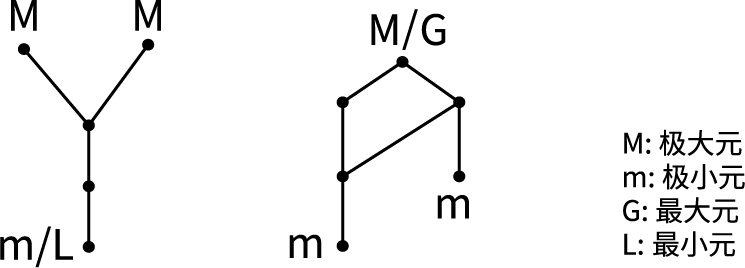
\includegraphics[width = 0.6\linewidth]{./images/maximal_greatest.png}
\end{figure} 

考虑 $ X = (0, 1) \subseteq \R $ 和小于等于关系 $ \leqslant $, $ X $ 没有极大元和最大元. 考虑 $ X = \set{\set{1}, \set{2}, \set{1, 2}} $ 和子集关系 $ \subseteq $, $ X $ 有唯一极大元 $ \set{1, 2} $ 和最大元 $ \set{1, 2} $. 设集合:
\[ A = \set{\set{n} \colon n, k \in \N, n \leqslant k} \,,\]

直观地说, $ A = \set{\set{0}, \set{1}, \set{2}, \dots, \set{k}} $.

那么考虑集合 $ A \cup \set{\varnothing} = \set{\varnothing, \set{0}, \set{1}, \dots, \set{k}} $. 这个偏序集 $ (A, \subseteq) $ 有 $ k + 1 $ 个极大元, $ 0 $ 个最大元.

由此看出:

\begin{proposition}
    $ X $ 为偏序集, 则 $ X $ 可能没有极大元, 或有任意个极大元. $ X $ 可能没有最大元或存在唯一最大元. 极小元和最小元同理.
\end{proposition}

\begin{proposition}
    若 $ X $ 为有限偏序集, 则 $ X $ 必然存在极大元和极小元.
\end{proposition}

\begin{proof}
    下面证明必然存在极大元, 极小元同理.

    归纳法. 若偏序集 $ X $ 为单元素集, 则其唯一元素为极大元. 归纳地假设任意 $ n $ 元素偏序集存在极大元, 要证明 $ n + 1 $ 元素偏序集存在极大元.

    设 $ X $ 为偏序集, $ |X| = n + 1 $, $ x \in X $. 则 $ X \setminus \set{x} $ 为 $ n $ 元素偏序集, 则 $ X \setminus \set{x} $ 存在极大元, 记为 $ m $. 现重新将 $ x $ 加入到 $ X \setminus \set{x} $ 中, 会出现三种情况: (1) $ m \le x $; (2) $ x \le m $; (3) $ x $, $ m $ 不可比.

    (1) 若 $ m \le x $: $ X \setminus \set{x} $ 中找不到比 $ m $ 大的元素, 也就找不到比 $ x $ 大的元素. 于是 $ X $ 中, 找不到比 $ x $ 大的元素, 则 $ x $ 成为新的极大元.

    (2) 若 $ x \le m $: 此时 $ X $ 中仍然找不到比 $ x $ 大的元素, 于是 $ m $ 仍是极大元.

    (3) 若 $ m $, $ x $ 不可比: 加入后 $ X $ 中仍然没有比 $ x $ 大的元素, 这不影响 $ m $ 仍是极大元.

    综上所述, 便完成了归纳. 于是对于任意有限偏序集, 总是存在极大元的.
\end{proof}

\begin{proposition}
    $ X $ 为偏序集, 若存在最大元, 则最大元是唯一的. 且此时极大元也是唯一的, 等于最大元. 也就是说, 最大元存在时, 极大元和最大元等价. 极小元和最小元同理.
\end{proposition}

\begin{remark}
    注意上面的逆命题并不成立, 若 $ X $ 有唯一极大元 $ x $, 则 $ x $ 不一定是 $ X $ 的最大元. (如果限制到有限的偏序集上, 情况如何?)

    针对这个逆命题, 我们可以举出反例, 定义集合 $ S_k \coloneqq \set{n \in \Z \colon 0 \leqslant n \leqslant k} $. 也就是说, $ S_k $ 为 $ 0 $ 到 $ k $ 的整数组成的集合:
    \[ \begin{array}{c}
        S_0 = \set{0} \\
        S_1 = \set{0, 1} \\
        S_2 = \set{0, 1, 2} \\
        S_n = \set{0, 1, 2, \dots, n}
    \end{array} \,.\]

    考虑集合 $ A = \set{S_n \colon n \in \N} \cup \set{\set{0, -1}} $, 即:
    \[ A = \set{\set{0, -1}, \set{0}, \set{0, 1}, \set{0, 1, 2}, \dots} \,.\]

    这是一个无限集, 其有唯一极大元 $ \set{0, -1} $, 但没有最大元.
\end{remark}

\begin{proof}
    设 $ (X, \le) $ 的一个子集 $ Y $ 存在最大元 $ m $. 假设存在另一个最大元 $ m' $, 按照定义 $ m, m' \in Y $, 且应该有 $ m \ge m' $ 和 $ m' \ge m $, 所以 $ m' = m $. 这说明最大元如果存在, 必然是唯一的.

    假设存在极大元 $ n $, $ n \in Y $, 所以有 $ m \ge n $.
    由于 $ m \in Y $, 所以要么 $ n \ge m $, 要么 $ n $ 和 $ m $ 不可比. 由于已经有 $ m \ge n $, 说明两者是可比的. 所以只可能 $ n \ge m $, 又有 $ m \ge n $, 则 $ m = n $. 这说明最大元存在时, 极大元是唯一等于最大元的.
\end{proof}

\begin{corollary}
    若 $ X $ 是一个有限的偏序集, 且 $ X $ 存在唯一极大元 $ x $, 则 $ x $ 就是 $ X $ 的最大元. 换句话说: $ X $ 存在最大元当且仅当 $ X $ 存在唯一极大元.
\end{corollary}

\begin{proof}
    设 $ X $ 是一个有限的 $ n $ 元偏序集, 其有唯一极大元 $ x $. 按照定义, $ \forall y \in X $, 要么 $ y \le x $, 要么两者不可比. 于是可以分出两种情况: (1) 对任意 $ y \in X $, 都有 $ y \le x $; (2) 存在 $ y \in X $, $ x $ 不可比.

    (1) 若所有 $ y \in X $ 都有 $ y \le x $: 按照定义, $ x $ 为最大元.

    (2) 若 $ X $ 中存在与 $ x $ 不可比的元素: 记作 $ y_1 $. 下面归纳地假设 $ X $ 中存在与 $ x $ 不可比的 $ y_i $. 要证明 $ X $ 中一定存在与 $ x $ 不可比的 $ y_{i + 1} > y_i $.

    首先一定存在 $ y_{i + 1} \in X $, $ y_{i + 1} > y_i $. 因为如果不存在此元素, 按照定义 $ y_i $ 成为极大元. 而 $ y_i $ 与 $ x $ 不可比, $ y_i \neq x $. 于是 $ X $ 有两个不同的极大元, 不符合题述唯一极大元的条件.

    其次 $ y_{i + 1} $ 和 $ x $ 一定是不可比的. 因为一旦可比, $ x \le y_{i + 1} $ 会导致 $ x $ 不是极大元; 而 $ y_{i + 1} \le x $ 会导致 $ y_i < y_{i + 1} \le x $ 即 $ y_i $ 和 $ x $ 可比.

    所以完成了归纳. 这意味着只要存在一个和 $ x $ 不可比的 $ y_1 \in X $, $ X $ 中就会存在无穷个元素 $ y_1, y_2, \dots $, 每个都是与 $ x $ 不可比的, 且这些元素互不相同: $ y_1 < y_2 < \cdots $. 但 $ X $ 是有限集, 这就产生了矛盾. 
    
    所以情况 (2) 是不存在的, 只有情况 (1) 成立, 此时 $ x $ 为最大元.
\end{proof}

\begin{proposition}
    $ X $ 为全序集, 则最大元和极大元始终等价. 极小元和最小元同理.
\end{proposition}

\begin{proof} 
    证明两部分: 最大元蕴含极大元; 极大元蕴含最大元.


    
\end{proof}

总结一下, 偏序集中: 极大元和最大元是两个不同的概念. 极大元可以有零个或任意个, 最大元只能有零个或一个. 且当最大元存在时, 两者等价, 此时两者都是唯一的.

而全序集中, 由于可比性: 最大元和极大元是始终等价的概念, 要么同时没有, 要么同时有唯一相同的最大元和极大元.

\paragraph{最大元和极大元的个数情况} \ 

偏序集中, 最大元和极大元有四种情况:
\begin{itemize}
    \item $ 0 $ 个极大元, $ 0 $ 个最大元
    \item $ 1 $ 个极大元, $ 0 $ 个最大元 (若偏序集有限, 不可能出现这种情况 ?)
    \item $ 1 $ 个极大元, $ 1 $ 个最大元
    \item 多个极大元, $ 0 $ 个最大元
\end{itemize}

全序集中, 最大元和极大元等价, 有两种情况:
\begin{itemize}
    \item $ 0 $ 个极大元, $ 0 $ 个最大元
    \item $ 1 $ 个极大元, $ 1 $ 个最大元
\end{itemize}


\subsubsection{上界与最小上界}
\begin{definition}[\text{上界 (upper bound)}]
    设 $ Y $ 是偏序集 $ X $ 的子集. 对于 $ \beta \in X $, 称 $ \beta $ 为 $ Y $ 的上界, 当且仅当 $ \forall y \in Y $, $ \beta \ge y $.
\end{definition}

若 $ \beta \in X $ 为 $ Y $ 的上界, 且 $ \beta $ 不在 $ Y $ 中, 则称 $ \beta $ 为 $ Y $ 的严格上界. 这等价于 $ \forall y \in Y $, $ y < \beta $.

\begin{definition}[\text{最小上界}]
    设 $ Y $ 是偏序集 $ X $ 的子集. 设 $ \beta \in X $ 为 $ Y $ 的上界, 称 $ \beta $ 为 $ Y $ 的最小上界, 当且仅当对于任意 $ Y $ 的上界 $ \beta' $ 满足 $ \beta \le \beta' $. 即 $ \beta $ 是所有上界的集合的最小元.
\end{definition}

同理可以定义下界 (lower bound) 和最大下界 (greatest lower bound).

\begin{remark}
    $ Y $ 的极大/小元和最大/小元都是 $ Y $ 中的元素, 而 $ Y $ 的上/下界和最小上界/最大下界却可以是 $ Y $ 外的元素.
\end{remark}

\begin{proposition}
    一个偏序集可以没有上界, 或存在任意个上界; 可以没有最小下界, 或存在唯一最小下界. 下界和最大下界同理.
\end{proposition}



\begin{proposition}
    设 $ Y $ 是偏序集 $ X $ 的子集. 若 $ \beta $ 为 $ Y $ 的一个上界, 若 $ \beta \in Y $, 则有下面两条结论:
    \begin{itemize}
        \item $ \beta $ 为 $ Y $ 的最小上界
        \item $ \beta $ 为 $ Y $ 的最大元
    \end{itemize}

    这就导出了最大元的等价定义: 若 $ Y $ 中存在元素等于最小上界, 则这个元素为最大元. 下界和最大下界同理.
\end{proposition}

\begin{proof}
    设 $ Y $ 是偏序集 $ X $ 的子集, $ \beta $ 为 $ Y $ 的一个上界且 $ \beta \in Y $. 由于 $ \beta $ 为上界, $ \forall y \in Y $, $ y \le \beta $. 由于 $ \beta \in Y $, 按照定义 $ \beta $ 为 $ Y $ 的最大元. 若 $ Y $ 还存在上界 $ \beta' $, 由于 $ \beta \in Y $, $ \beta \le \beta' $. 所以 $ \beta $ 为最小上界.
\end{proof}

就此我们可以导出最小上界性质 (最大下界同理).

\begin{proposition}[\text{最小上界性质}]
    设 $ Y $ 是偏序集 $ X $ 的子集, $ \beta $ 为 $ Y $ 的最小上界. 若 $ y \in Y $ 且 $ y < \beta $, 则存在 $ y' \in Y $ 满足 $ y < y' \le \beta $.
\end{proposition}

\begin{proof}
    假设对于给定 $ y < \beta $, 找不到 $ y' \in Y $ 使得 $ y < y' \le \beta $. 这等价于对于任意 $ y' \in Y $, 有 $ y' \le y $ 或 $ y' > \beta $. 对于前者, 所有的 $ y' \in Y $ 都有 $ y' \le y $, 则 $ y $ 为上界, 而 $ y $ 小于最小上界 $ \beta $, 这产生了矛盾. 后者也是不可能的, 因为 $ \beta $ 为上界, $ y' \le \beta $. 综上所述, 一定存在 $ Y $ 中的元素 $ y' $ 满足 $ y < y' \le \beta $.
\end{proof}


\subsection{良序集}
\begin{definition}[\text{良序集}]
    设 $ Y $ 为偏序集 $ X $ 的子集. 称 $ Y $ 是良序集 (well-ordered set, woset), 当且仅当 $ Y $ 的每个非空子集都存在最小元 $ \min(Y) $
\end{definition}

\begin{remark}
    空集 $ \varnothing $ 是良序集. 因为其每个非空子集都存在最小元是一个空真的命题.
\end{remark}


\paragraph{例}
$ \N $ 是良序的; $ \Z $, $ \Q $, $ \R $ 都不是良序的.

\begin{proposition}
    良序集的子集也是良序集.
\end{proposition}

\begin{proof}
    设 $ X $ 为良序集, $ Y \subseteq X $. 若 $ Y $ 为空集, 则 $ Y $ 自然为良序集. 若 $ Y $ 非空, 考虑任意非空子集 $ Y' \subseteq Y \subseteq X $. 由于 $ Y' $ 是 $ X $ 的非空子集, 所以 $ Y' $ 有最小元. 故 $ Y $ 为良序集.
\end{proof}

\begin{remark}
    因此, 偏序集、全序集、良序集的子集仍然分别为偏序集、良序集、全序集. 故子集保留原集的序.
\end{remark}

\begin{proposition}
    有限的全序集是良序集.
\end{proposition}

\begin{proof}
    使用归纳法. 设 $ X $ 为一个有限的全序集. 若 $ X $ 为单元素集, 则显然$ X $ 只有一个非空子集, 且其存在最小元素. 于是 $ X $ 为良序集, 这证明了基础情形. 下面归纳地假设有限的 $ n $ 元全序集为良序集, 要证明 $ n + 1 $ 元全序集也为良序集. 
    
    设 $ X $ 为一个 $ n + 1 $ 元全序集. 取其中一个元素 $ x $, 则 $ X \setminus \set{x} $ 为良序集. 现在将 $ x $ 加入到 $ X \setminus \set{x} $ 中, 考虑任意非空 $ Y \subseteq X $, 则其可能包含新加进去的 $ x $. 于是分两种情况讨论: 
    
    若 $ x \notin Y $, 则 $ Y \subseteq X \setminus \set{x} $, 也就为良序集, 有最小元.
    
    若 $ x \in Y $, 则 $ Y \setminus \set{x} \subseteq X \setminus \set{x} $, 也就为良序集, 有最小元 $ m $. 由于 $ Y \subseteq X $ 为全序集, $ Y $ 中加入的 $ x $ 与 $ m $ 有两种情况: $ x \le m $ 或 $ m \le x $. 前者 $ x $ 成为新的最小元, 后者 $ m $ 仍为最小元. 

    综上所述, 如果 $ n $ 元素全序集是良序集. 则 $ n + 1 $ 元素全序集的任意非空子集都存在最小元, 于是为良序集.
\end{proof}

\begin{remark}
    同理还可以证明: 全序集的有限子集存在最大元.
\end{remark}

良序集的重要性质在于, 可以在其上使用归纳法.

\begin{proposition}[\text{强归纳原理}]
    设 $ (X, \le) $ 为良序集, $ P(n) $ 是关于 $ n \in X $ 的命题. 若满足: ``对所有 $ m < n $, $ P(m) $ 成立, 则 $ P(n) $ 成立.'' 则 $ P(n) $ 对一切 $ n \in X $ 皆成立.
\end{proposition}

\begin{remark}
    注意, 此处无需说明基础情形. 因为对于 $ X $ 的最小元 $ m_0 $, $ P(m_0) $ 是空真的.
\end{remark}

\begin{proof}
    假设对于所有 $ m < n $, $ P(m) $ 成立, 则 $ P(n) $ 成立; 但存在 $ n \in X $, $ P(n) $ 不成立. 我们将所有使 $ P(n) $ 不成立的元素装在集合中:
    \[ A \coloneqq \set{n \in X \colon P(n) \text{ 为假}} \,.\]

    显然有 $ A \subseteq X $ 且 $ A $ 非空. 由于 $ X $ 为良序集, 所以 $ A $ 必然存在最小元, 记为 $ n_0 $. 那么对于任意 $ x < n_0 $, $ x \notin A $, 即 $ P(x) $ 成立. 于是根据归纳假设, $ P(n_0) $ 也成立, 这和 $ n_0 \in A $ 矛盾.
\end{proof}

\begin{lemma}
    设 $ (X, \le) $ 为偏序集, $ x_0 \in X $. 则存在 $ X $ 的良序子集 $ Y $, 它以 $ x_0 $ 为最小元, 且没有严格上界.
\end{lemma}

由该引理可以导出一个重要推论.

\begin{lemma}[\text{Zorn 引理 / 超限归纳原理}]
    非空偏序集 $ X $ 的每个全序子集 $ Y $ 都有上界, 那么 $ X $ 存在极大元.
\end{lemma}



\end{document}